\chapter{\textit{Filter Bank Multicarrier} - FBMC} \label{capitulo3}

%Este capítulo descreve as principais formas de onda candidatas a 5G. O OFDM já é bastante conhecido, então será apresentado de forma breve, dando-se destaque as suas variações, citadas no capítulo anterior. O FBMC e o UFMC são trazidos de forma detalhada, mostrando-se, inclusive, o comportamento dessas formas de onda sob efeitos do canal de comunicação RF. 

%\section{Orthogonal Fequency Division Multiplexing (OFDM)}

%\begin{figure}[h!]
%\centering
%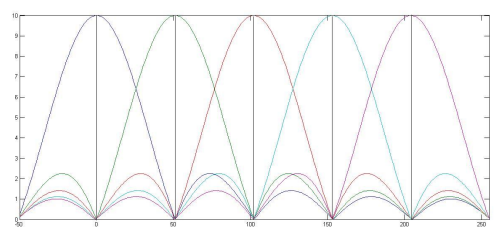
\includegraphics[width=3.5in]{fig_OFDM_freq.png}
%\caption{Subportadoras OFDM}
%\label{fig_OFDM_freq.png}
%\end{figure}
%\end{figure}

%\section{Filter Bank Multi Carrier (FBMC)}
A descrição da forma de onda FBMC pode ser vista como uma generalização do OFDM, com menos restrições em relação ao formato de pulso utilizado para filtrar subportadoras. No contexto da 5G, entretanto, trata-se de algo mais robusto. O projeto PHYDAS (\textit{\textbf{PHY}sical layer for \textbf{DY}namic \textbf{A}cces\text{S} and cognitive radio}) \cite{phydas} se preocupou em criar um desenho bastante específico desta tecnologia, procurando construí-la de tal forma que diversas desvantagens do OFDM fossem superadas, abrindo portas para tornar as aplicações idealizadas para a 5G possíveis. É esta versão que será trazida aqui. 


\section{O Formato de Pulso}\label{pulso} 

Como o filtro FBMC é o que o diferencia do OFDM, inicia-se a apresentação da forma de onda através do formato de pulso utilizado. Sabe-se que a IFFT/FFT possui um efeito de filtragem dos sinais a que é aplicada \cite{Boroujeny}. No domínio do tempo (discreto), pode-se representar este efeito da maneira a seguir \cite{Bellanger}:
\begin{equation}
y_{n} = \frac{1}{M}[x(n-M)+...+x(n-1)] = \frac{1}{M}\sum_{i=1}^{M}x(n-1),
\end{equation}
um filtro passa-baixa do tipo FIR (\textit{finite impulse response} - reposta ao impulso finita). No domínio da frequência \cite{Bellanger}:
\begin{equation}\label{eq_freq}
I(f) = \frac{sin\pi fM}{Msin\pi f}
\end{equation}

A equação \ref{eq_freq} é a fórmula matemática que leva ao espectro visto na figura \ref{fig_OFDM_freq}. A existências de lóbulos laterais de relativamente alta potência esbarra em algumas características que a forma de onda que transmitirá sinais 5G precisará ter. Recapitulando, isto é prejudical a sinais assíncronos, visto que representam um alto potencial para gerar interferências e assincronismo será fundamental no contexto da IoT \cite{Wunder}.  
\par Pensando nisso, procurou-se criar um tipo de filtro mais adequado. Baseou-se a escolha do pulso no critério de Nyquist, que no domínio da frequência significa simetria em relação a frequência de corte \cite{Bellanger}. 
\par Focando agora no processo de transmissão e recepção, para que este ocorra livre de erros, o filtro que transmite deve estar casado com aquele que recebe o sinal. Assim, utiliza-se "meio filtro" de Nyquist na saída e outro "meio filtro" na entrada. 
\par Com esses critérios em mente, desenhou-se alguns possíveis formatos para o pulso FBMC, chegando-se aos coeficientes abaixo: 

\begin{center} \label{coef_FBMC}
\begin{tabular}{ c c c c c c  }
 K & $H_{0}$ &  $H_{1}$ & $H_{2}$ & $H_{3}$ & $\sigma^{2}$ (dB) \\ 
 2 & 1 & $\frac{\sqrt{2}}{2}$ & - & - & -35\\  
 3 & 1 & 0.911438 & 0.411438 & - & -44\\
 4 & 1 & 0.971960 & $\frac{\sqrt{2}}{2}$ & 0.235147 & -65
\end{tabular}
\end{center}

Na tabela \ref{coef_FBMC}m, K representa o fator de superposição, ou seja, quantas amostras se sobrepõem em cada versão do filtro. Quanto maior for K, melhor localizado na frequência será o pulso. Para K = 4, tem-se a resposta da figura \ref{fig_FBMC}, no domínio da frequência:

\begin{figure}[h!]
\centering
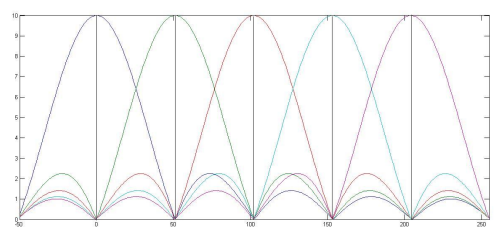
\includegraphics[width=3.5in]{fig_OFDM_freq.png}
\caption{Subportadoras FBMC}
\label{fig_FBMC}
\end{figure}

\par Nota-se uma expressiva redução da amplitude dos lóbulos laterais \cite{Bellanger}, um excelente benefício no contexto M2M. Em termos matemáticos, a forma de pulso se traduz em\cite{Bellanger}: 

\begin{equation}\label{eq_freq}
H(f) = \sum_{k=-(K-1)}^{K-1}H_{k}\frac{\sin(\pi(f-\frac{k}{MK}))}{MKsin(\pi(f-\frac{k}{MK}))}
\end{equation}

\par O próximo passo na construção da forma de onda FBMC é criar múltiplas subportadoras como a da \ref{fig_FBMC}, centralizadas em diferentes frequências. Isto é feito como mostra o diagrama de blocos da figura \ref{Trans_FBMC}. 

\begin{figure}[h!]
\centering
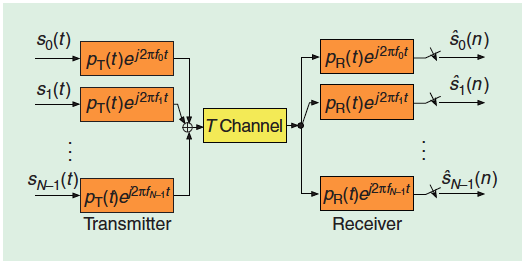
\includegraphics[width=3.5in]{Trans_FBMC.png}
\caption{Diagrama do Modem FBMC \cite{Boroujeny}}
\label{Trans_FBMC}
\end{figure}

\par Na seção do OFDM viu-se o quanto os algortimos de IFFT/FFT foram fundamentais no desenvolvimento da forma de onda tratada ali. Observando-se a Figura \ref{Trans_FBMC}, observa-se uma oportunidade de utilização da ferramenta, já que cada ramo é multiplicado por $\exp^{^{+}_{-} j2\pi}{f_{k}}$, $f_{k} = \frac{ft}{T}$ - coeficientes da transformada de Fourier. 

\par A próxima seção mostra que de fato se pode utilizar a transformada de Fourier para gerar os símbolos FBMC, o que torna a implementação muito mais simples. Para tanto é utilizada um recurso chamado "filtro polifásico". No caso da Figura \ref{Trans_FBMC}, seria necessária a utilização de osciladores de frequência, o que pode dificultar o processo de recepção correta, visto que instrumentos deste tipo são bastante suscetíveis a erros. 

\section{Filtros Polifásicos}

Filtros polifásicos são uma estrutura bastante comum em processamento digital de sinais. Qualquer sequência pode ser dividia em subsequências de menor ordem. Consideremos, por exemplo, a sequência h[n], que pode representar um filtro FIR (\textit{finite impulse response} - resposta ao impulso finita). Suas componentes polifásicas $h_{m}$ são dadas por:

\begin{equation}
h_{m}[Mn] = h[Mn + m],
\end{equation}

em que $m$ é uma sequência tal que $-\infty < m < \infty$, assim como $n$ e $M$ é um inteiro positivo. 
\par Essa estrutura tão simples parece não trazer benefício algum. Isto é um grande engano. Dentro do contexto de criação de sinais FBMC, esta ferramenta será bastante importante e possibilitará a redução da complexidade de implementação do sinal.

\par Imagine o processo de criação de um símbolo FBMC. Esta forma de onda é um tipo de sinal FDM (\textit{frequency division multiplexing} - multiplexação por divisão na frequência). Isto significa que um conjunto de símbolos de banda larga 
$B$ será dividido em outros sinais, de mesma largura de banda $B' < B$. Esta característica é exibida na Figura \ref{espectro FDM}

\begin{figure}[h!]
\centering
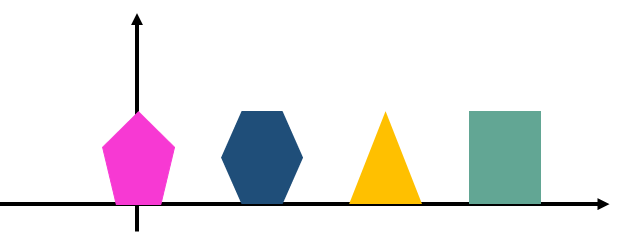
\includegraphics[width=4.5in]{Filtrado.png}
\caption{Sinal FDM Genérico}
\label{espectro FDM}
\end{figure}

\par A maneira convencional de gerar esse tipo de sinal implica em replicação de hardware no processo de recepção, o que amplia os custos, o consumo de energia e também o uso de espaço físico para acomadar as peças necessárias \cite{Krishna}. É por isso que o processamento digital do sinal é importante, tanto na geração do sinal quanto na sua recuperação. É aqui que entram as componentes polifásicas, em conjunto com alguns recursos extras que também serão bastante importantes, conforme será visto a seguir.
\par As próximas explanações são baseadas na referência \cite{Krishna}. Neste artigo, o autor traz o conceito de filtros polifásicos associado ao processo de recepção de um sinal FDM. Aqui, será tratado o processo de geração do símbolo FBMC.
\par Por se tratar de um esquema de múltiplos canais, o primeiro passo na criação de um símbolo FBMC é dividir uma sequência longa de símbolos modulados em subsequências menores: 

\begin{figure}[h!]
\centering
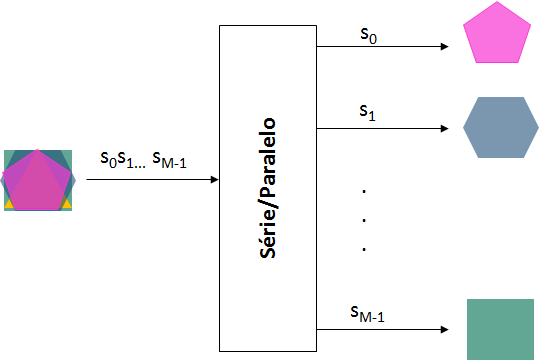
\includegraphics[width=3.5in]{serie_paralelo.png}
\caption{Divisão do Sinal FBMC em Sub-bandas}
\label{espectro super FDM}
\end{figure}

\par Cada sub-banda deve ser levada à frequência desejada e filtrada com o formato de pulso adequado. Por brevidade, aqui os filtros serão supostos retangulares, mas sabe-se que a forma adequada é aquela apresentada na seção \ref{pulso}. Estes passos são mostrados a seguir:

\begin{figure}[h!]
\centering
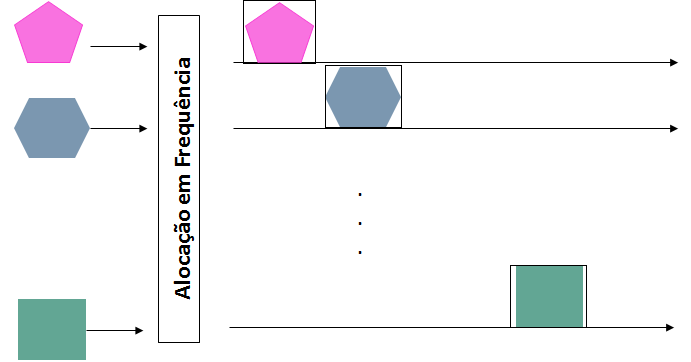
\includegraphics[width=3.5in]{freq_aloc.png}
\caption{Alocação na Frequência e Filtragem}
\label{filtro_freq}
\end{figure}

\par A estrutura que torna esse processo possível é exibida na figura

\begin{figure}[h!]
\centering
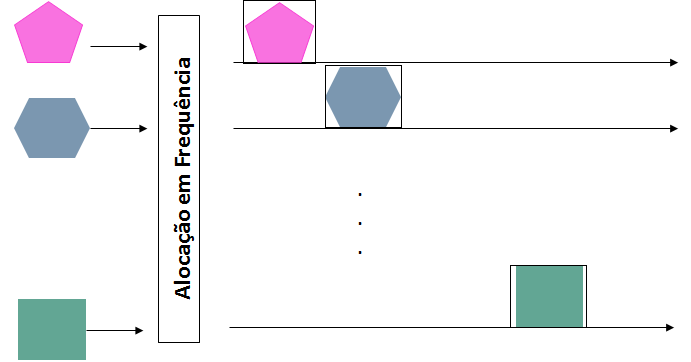
\includegraphics[width=3.5in]{freq_aloc.png}
\caption{Alocação na Frequência e Filtragem}
\label{filtro_freq}
\end{figure}


\par Imagine um sinal super-amostrado $x_{u}[n]$ do domínio do tempo por um fator M inteiro. Ele será dado pela equação \ref{compoli}

\begin{equation}]\label{compoli}
x_{u}[n] = x[n/M],
\end{equation}

No domínio da frequência, este sinal será representado por

\begin{equation}
X_{u}(e^{j\omega}) = M/T\sum{r=-\infty}^{\infty}X_{c}\bigg[j\bigg(\frac{M\omega}{T}-\frac{2\pi rM}{T}\bigg)\bigg]
\end{equation}

Graficamente, isto consiste em repetir o sinal M vezes no espectro de forma periódica, sendo que a largura de banda de cada repetição é M vezes mais estreita e a amplitude M vezes maior. Se $x_{u}$ fosse o símbolo FDM da Figura \ref{espectro FDM}, teríamos uma repetição de múltiplas larguras de banda, e consequentemente a sobreposição. A figura \ref{espectro super FDM} ilustra isto. 

\begin{figure}[h!]
\centering
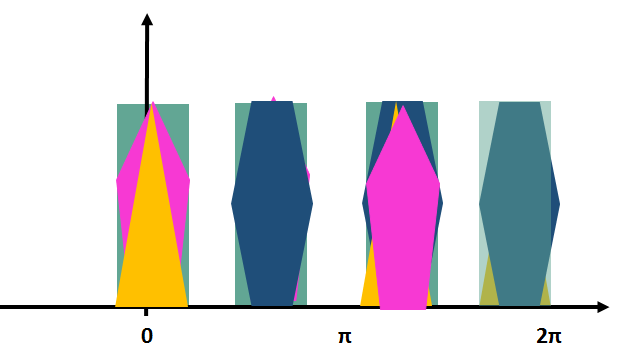
\includegraphics[width=4.5in]{Super_Amostrado_1.png}
\caption{Sinal FDM Super Amostrado}
\label{espectro super FDM}
\end{figure}

\par No contexto FBMC, parte-se de uma banda contínua e se deseja chegar a algo parecido com a Figura \ref{espectro FDM}: 

\begin{figure}[h!]
\centering
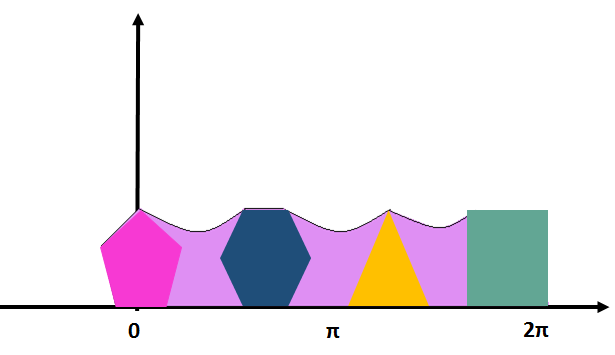
\includegraphics[width=4.5in]{Espetro_FBMC.png}
\caption{Sinal FBMC}
\label{espectro super FDM}
\end{figure}

\par Seja $h[n]$ o PHYDAS apresentado na seção \label{pulso} e $h_{m}$ suas componentes polifásicas, pode-se contruir a seguinte estrutura: 






\section{Transmissor/Receptor FBMC}
\subsection{Modulação O-QAM} 



\section{Desempenho sob o efeito de não linearidades }